\documentclass[12pt,a4paper]{article}

% ─── Page Layout ───────────────────────────────────────────────────────────────
\usepackage[a4paper, margin=0.8in, headheight=14pt]{geometry}

% ─── Fonts (XeLaTeX) ───────────────────────────────────────────────────────────
\usepackage{fontspec}
\usepackage{unicode-math}
\setmainfont{TeX Gyre Pagella}
\setmonofont[Scale=0.88]{TeX Gyre Cursor}
\setmathfont{Latin Modern Math}

% ─── Packages ──────────────────────────────────────────────────────────────────
\usepackage{xcolor}
\usepackage{colortbl}
\usepackage{titlesec}
\usepackage{enumitem}
\usepackage{tabularx}
\usepackage{booktabs}
\usepackage{array}
\usepackage{amsmath}
\usepackage{tikz}
\usetikzlibrary{shapes.geometric, arrows.meta, positioning, calc, fit, decorations.pathreplacing}
\usepackage{tcolorbox}
\tcbuselibrary{skins, breakable}
\usepackage{hyperref}
\usepackage{fancyhdr}
\usepackage{graphicx}
\usepackage{microtype}
\hyphenpenalty=10000
\exhyphenpenalty=10000
\sloppy
\usepackage{caption}
\usepackage{setspace}
\usepackage{multirow}
\usepackage{tocloft}

% ─── Q&A helper ────────────────────────────────────────────────────────────────
\newcommand{\Q}[1]{\textbf{#1}\par\noindent\ignorespaces}

% ─── Colour Palette ────────────────────────────────────────────────────────────
\definecolor{myred}{RGB}{196,30,58}
\definecolor{mydark}{RGB}{30,30,50}
\definecolor{mygreen}{RGB}{14,120,80}
\definecolor{myteal}{RGB}{0,130,140}
\definecolor{myamber}{RGB}{180,100,0}
\definecolor{mypurple}{RGB}{100,30,160}
\definecolor{mygray}{RGB}{246,247,249}
\definecolor{mgframe}{RGB}{180,185,200}
\definecolor{watermark}{RGB}{145,150,170}
\definecolor{hdrred}{RGB}{250,232,235}
\definecolor{hdrgreen}{RGB}{220,244,233}
\definecolor{hdrteal}{RGB}{220,242,244}
\definecolor{hdramber}{RGB}{253,242,215}
\definecolor{hdrpurple}{RGB}{238,228,255}
\definecolor{hdrgray}{RGB}{238,240,245}
\definecolor{rowalt}{RGB}{250,251,253}

% ─── Section Formatting ────────────────────────────────────────────────────────
\titleformat{\section}
  {\large\bfseries\color{myred}}{\thesection.}{0.5em}{}
  [\vspace{1pt}{\color{myred}\rule{\linewidth}{0.8pt}}]
\titleformat{\subsection}
  {\normalsize\bfseries\color{myteal}}{\thesubsection}{0.5em}{}
\titlespacing*{\section}{0pt}{18pt}{7pt}
\titlespacing*{\subsection}{0pt}{11pt}{4pt}

% ─── Paragraph ─────────────────────────────────────────────────────────────────
\setlength{\parindent}{0pt}
\setlength{\parskip}{4pt}

% ─── TOC Styling ───────────────────────────────────────────────────────────────
\renewcommand{\cfttoctitlefont}{\large\bfseries\color{myred}}
\renewcommand{\cftaftertoctitle}{\par\noindent{\color{myred}\rule{\linewidth}{0.8pt}}}
\setlength{\cftbeforetoctitleskip}{0pt}
\setlength{\cftaftertoctitleskip}{6pt}
\renewcommand{\cftsecfont}{\normalsize\bfseries\color{mydark}}
\renewcommand{\cftsecpagefont}{\normalsize\bfseries\color{mydark}}
\renewcommand{\cftsecleader}{\cftdotfill{\cftdotsep}}
\setlength{\cftbeforesecskip}{7pt}
\renewcommand{\cftsubsecfont}{\small\color{mydark}}
\renewcommand{\cftsubsecpagefont}{\small\color{mydark}}
\setlength{\cftbeforesubsecskip}{3pt}
\setlength{\cftsubsecindent}{1.4em}

% ─── Table helpers ─────────────────────────────────────────────────────────────
\renewcommand{\arraystretch}{1.45}
\setlength{\tabcolsep}{6pt}
\arrayrulecolor{mydark}
\newcolumntype{B}[1]{>{\small\bfseries\raggedright\arraybackslash}m{#1}}
\newcolumntype{Y}{>{\small\raggedright\arraybackslash}X}
\renewcommand{\tabularxcolumn}[1]{m{#1}}

% ─── Header / Footer ───────────────────────────────────────────────────────────
\pagestyle{fancy}
\fancyhf{}
\fancyhead[L]{\small\color{myred}\textbf{PE-EC702C}\;\color{mydark}--- Neural Network and Fuzzy Logic Control}
\fancyhead[R]{\small\color{myteal}\textbf{Module 1 Notes}}
\fancyfoot[C]{\small\color{mydark}\thepage}
\fancyfoot[R]{\small\color{watermark}\textit{\copyright\ Biraj}}
\renewcommand{\headrulewidth}{0.5pt}
\renewcommand{\footrulewidth}{0.3pt}

% ─── Hyperref ──────────────────────────────────────────────────────────────────
\hypersetup{
  colorlinks=true, linkcolor=myteal, urlcolor=myteal,
  pdfauthor={Biraj Sarkar},
  pdftitle={PE-EC702C --- Module 1 Notes}
}

% ─── tcolorbox styles ──────────────────────────────────────────────────────────
\tcbset{
  tikzbox/.style={
    colback=mygray, colframe=mgframe, boxrule=0.6pt, arc=4pt,
    left=8pt, right=8pt, top=6pt, bottom=6pt,
    colbacktitle=mgframe, coltitle=mydark,
    fonttitle=\small\bfseries
  },
  defbox/.style={
    colback=hdrgreen, colframe=mygreen, boxrule=0.8pt, arc=4pt,
    left=9pt, right=9pt, top=6pt, bottom=6pt,
    colbacktitle=mygreen, coltitle=white,
    fonttitle=\small\bfseries
  },
  formulabox/.style={
    colback=hdrteal, colframe=myteal, boxrule=0.8pt, arc=4pt,
    left=9pt, right=9pt, top=7pt, bottom=7pt,
    colbacktitle=myteal, coltitle=white,
    fonttitle=\small\bfseries
  },
  examplebox/.style={
    colback=hdramber, colframe=myamber, boxrule=0.8pt, arc=4pt,
    left=9pt, right=9pt, top=6pt, bottom=6pt,
    colbacktitle=myamber, coltitle=white,
    fonttitle=\small\bfseries,
    breakable
  },
  masonbox/.style={
    colback=hdrpurple, colframe=mypurple, boxrule=0.8pt, arc=4pt,
    left=9pt, right=9pt, top=6pt, bottom=6pt,
    colbacktitle=mypurple, coltitle=white,
    fonttitle=\small\bfseries
  },
  exambox/.style={
    colback=hdrpurple, colframe=mypurple, boxrule=1pt, arc=5pt,
    left=10pt, right=10pt, top=8pt, bottom=8pt,
    colbacktitle=mypurple, coltitle=white,
    fonttitle=\bfseries,
    breakable, title after break={\textbf{Frequently Asked / Viva Questions (contd.)}}}
}
\tcbset{breakable}

% ─── TikZ styles ───────────────────────────────────────────────────────────────
\tikzset{
  block/.style={rectangle, draw=myteal, fill=hdrteal,
    text width=2.2cm, align=center, minimum height=0.85cm,
    font=\small, rounded corners=3pt, line width=0.7pt},
  arrow/.style={-Stealth, thick, color=mydark},
  line/.style={thick, color=mydark}
}

% ═══════════════════════════════════════════════════════════════════════════════
\begin{document}
% ═══════════════════════════════════════════════════════════════════════════════

\begin{center}
  {\LARGE\bfseries\color{myred} PE-EC702C --- Neural Network \& Fuzzy Logic Control}\\[5pt]
  {\normalsize\color{mydark} Semester VII \quad$\bullet$\quad 3L:0T:0P \quad$\bullet$\quad 3 Credits}\\[3pt]
  {\normalsize\color{myteal}\textbf{Module 1 Exam Notes: Neural Networks and Pattern Association}}\\[3pt]
  {\small\color{mydark} CGEC \;$|$\; B.Tech ECE (2023--27) \;$|$\; \textit{Biraj Sarkar}}
\end{center}
\vspace{2pt}
\noindent{\color{myred}\rule{\linewidth}{1.5pt}}
\vspace{2pt}

\hypersetup{linkcolor=mydark}
\tableofcontents
\hypersetup{linkcolor=myteal}
\newpage

% ===============================================================================
\section{Biological vs. Artificial Neural Networks}
% ===============================================================================

An Artificial Neural Network (ANN) is an information-processing paradigm inspired by the structure and functional aspects of biological neural systems.

\begin{tcolorbox}[defbox, title={Artificial Neural Network (ANN)}]
An \textbf{Artificial Neural Network (ANN)} is a parallel, distributed computational model consisting of simple processing units (neurons) interconnected by weighted links, designed to learn patterns and relationships from data.
\end{tcolorbox}

\subsection{Structural and Functional Mapping}
The biological brain consists of billions of highly interconnected cells called neurons. The artificial neuron models this biological mechanism:

\begin{tcolorbox}[tikzbox, title={Biological vs. Artificial Neuron Mapping}]
\centering
\begin{minipage}{0.48\textwidth}
  \centering
  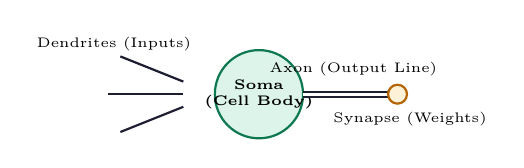
\begin{tikzpicture}[scale=0.8, every node/.style={font=\tiny}]
    % Dendrites
    \draw[thick, color=mydark] (-2.2, 0.6) -- (-1.2, 0.2);
    \draw[thick, color=mydark] (-2.2, -0.6) -- (-1.2, -0.2);
    \draw[thick, color=mydark] (-2.4, 0) -- (-1.2, 0);
    \node at (-2.3, 0.8) {Dendrites (Inputs)};
    
    % Soma
    \draw[thick, fill=hdrgreen, draw=mygreen] (0,0) circle (0.7cm);
    \node[align=center] at (0,0) {\textbf{Soma}\\\textbf{(Cell Body)}};
    
    % Axon
    \draw[line, double, double distance=1pt] (0.7, 0) -- (2.2, 0);
    \node at (1.5, 0.4) {Axon (Output Line)};
    
    % Synapse
    \draw[thick, fill=hdramber, draw=myamber] (2.2, 0) circle (0.15cm);
    \node at (2.4, -0.4) {Synapse (Weights)};
  \end{tikzpicture}
  \par\vspace{2pt}\small\textbf{Biological Neuron Elements}
\end{minipage}
\hfill
\begin{minipage}{0.48\textwidth}
  \centering
  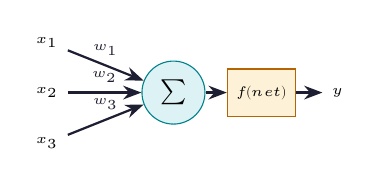
\begin{tikzpicture}[scale=0.8, every node/.style={font=\tiny}]
    % Inputs
    \node (x1) at (-2.0, 0.8) {$x_1$};
    \node (x2) at (-2.0, 0) {$x_2$};
    \node (x3) at (-2.0, -0.8) {$x_3$};
    
    % Summing junction
    \node[circle, draw=myteal, fill=hdrteal, minimum size=0.8cm, font=\small] (sum) at (0,0) {$\sum$};
    
    % Weights
    \draw[arrow] (x1) -- node[midway, above] {$w_1$} (sum);
    \draw[arrow] (x2) -- node[midway, above] {$w_2$} (sum);
    \draw[arrow] (x3) -- node[midway, above] {$w_3$} (sum);
    
    % Activation
    \node[rectangle, draw=myamber, fill=hdramber, minimum height=0.6cm, minimum width=0.8cm] (act) at (1.4, 0) {$f(net)$};
    \draw[arrow] (sum) -- (act);
    
    % Output
    \node (y) at (2.6, 0) {$y$};
    \draw[arrow] (act) -- (y);
  \end{tikzpicture}
  \par\vspace{2pt}\small\textbf{Artificial Neuron Model}
\end{minipage}
\end{tcolorbox}

\par\noindent
The physical correspondences between biological and artificial components are summarized below:
\par\noindent
{\renewcommand{\arraystretch}{1.9}%
\begin{tabularx}{\linewidth}{|>{\bfseries}B{3.5cm}|Y|Y|}
\hline
Biological Component & Artificial Equivalent & Functional Role \\
\hline
Dendrites & Inputs ($x_i$) & Receives signals from other neurons \\[4pt]
\hline
Soma (Cell Body) & Summing Junction ($\sum$) & Aggregates all incoming weighted inputs \\[6pt]
\hline
Axon & Output Transmission Line & Carries the output activation signal \\
\hline
Synapse & Weights ($w_i$) & Regulates the strength of connections \\[4pt]
\hline
Synaptic Threshold & Activation Function ($f$) & Determines output state based on total input \\
\hline
\end{tabularx}}

% ===============================================================================
\section{Typical Architectures of ANNs}
% ===============================================================================

Neural network topologies are broadly classified into three categories based on the flow of signals and feedback loops:

\begin{enumerate}[leftmargin=*, itemsep=4pt]
  \item \textbf{Single-Layer Feedforward Network:} Consists of an input layer of source nodes that connects directly to an output layer of neurons. There are no feedback loops and no hidden layers. (Example: Hebb net, Perceptron, Adaline).
  \item \textbf{Multi-Layer Feedforward Network:} Contains one or more hidden layers of processing units between the input and output layers. This architecture enables the network to learn non-linear decision boundaries. (Example: Backpropagation MLP).
  \item \textbf{Recurrent (Feedback) Network:} Contains at least one feedback loop where output signals are fed back as inputs to neurons in previous or current layers. (Example: Hopfield Network, BAM).
\end{enumerate}

% ===============================================================================
\section{Common Activation Functions}
% ===============================================================================

Activation functions (transfer functions) introduce non-linearity into the neuron model, allowing it to solve complex, non-linear problems.

\begin{tcolorbox}[formulabox, title={Mathematical Formulations of Activation Functions}]
Let $net = \sum w_i x_i + b$ be the net input to the neuron.
\par\vspace{4pt}
{\renewcommand{\arraystretch}{1.9}%
\begin{tabularx}{\linewidth}{B{3.2cm} Y B{3.8cm}}
\hline
Function & Mathematical Form & Range \\[4pt]
\hline
Binary Step & $f(net) = \begin{cases} 1 & \text{if } net \ge 0 \\ 0 & \text{if } net < 0 \end{cases}$ & $\{0, 1\}$ \\[8pt]
\hline
Bipolar Step & $f(net) = \begin{cases} 1 & \text{if } net \ge 0 \\ -1 & \text{if } net < 0 \end{cases}$ & $\{-1, 1\}$ \\[8pt]
\hline
Binary Sigmoid & $f(net) = \frac{1}{1 + e^{-\lambda net}}$ & $(0, 1)$ \\[6pt]
\hline
Bipolar Sigmoid & $f(net) = \frac{2}{1 + e^{-\lambda net}} - 1 = \tanh\left(\frac{\lambda net}{2}\right)$ & $(-1, 1)$ \\[6pt]
\hline
Rectified Linear (ReLU) & $f(net) = \max(0, net)$ & $[0, \infty)$ \\[4pt]
\hline
\end{tabularx}}
\end{tcolorbox}

\begin{tcolorbox}[tikzbox, title={Activation Function Shapes}]
\centering
\begin{minipage}{0.23\textwidth}
  \centering
  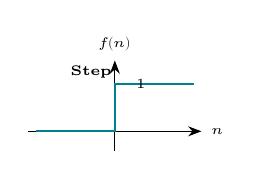
\begin{tikzpicture}[scale=0.5]
    \draw[-Stealth] (-2.2,0) -- (2.2,0) node[right] {\tiny $n$};
    \draw[-Stealth] (0,-0.5) -- (0,1.8) node[above] {\tiny $f(n)$};
    \draw[thick, color=myteal] (-2.0, 0) -- (0, 0) -- (0, 1.2) -- (2.0, 1.2);
    \node at (0.3, 1.2) [right] {\tiny $1$};
    \node at (-0.6, 1.5) {\textbf{\tiny Step}};
  \end{tikzpicture}
\end{minipage}
\hfill
\begin{minipage}{0.23\textwidth}
  \centering
  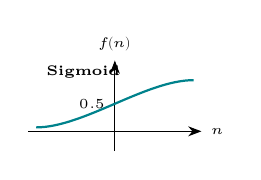
\begin{tikzpicture}[scale=0.5]
    \draw[-Stealth] (-2.2,0) -- (2.2,0) node[right] {\tiny $n$};
    \draw[-Stealth] (0,-0.5) -- (0,1.8) node[above] {\tiny $f(n)$};
    \draw[thick, color=myteal] (-2.0, 0.1) .. controls (-0.8, 0.1) and (0.8, 1.3) .. (2.0, 1.3);
    \node at (0, 0.7) [left] {\tiny $0.5$};
    \node at (-0.8, 1.5) {\textbf{\tiny Sigmoid}};
  \end{tikzpicture}
\end{minipage}
\hfill
\begin{minipage}{0.23\textwidth}
  \centering
  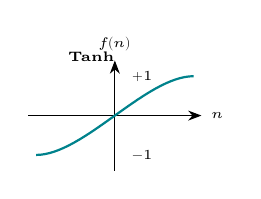
\begin{tikzpicture}[scale=0.5]
    \draw[-Stealth] (-2.2,0) -- (2.2,0) node[right] {\tiny $n$};
    \draw[-Stealth] (0,-1.4) -- (0,1.4) node[above] {\tiny $f(n)$};
    \draw[thick, color=myteal] (-2.0, -1.0) .. controls (-0.8, -1.0) and (0.8, 1.0) .. (2.0, 1.0);
    \node at (0.2, 1.0) [right] {\tiny $+1$};
    \node at (0.2, -1.0) [right] {\tiny $-1$};
    \node at (-0.6, 1.5) {\textbf{\tiny Tanh}};
  \end{tikzpicture}
\end{minipage}
\hfill
\begin{minipage}{0.23\textwidth}
  \centering
  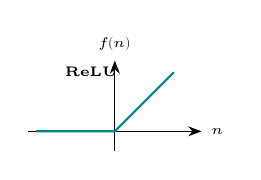
\begin{tikzpicture}[scale=0.5]
    \draw[-Stealth] (-2.2,0) -- (2.2,0) node[right] {\tiny $n$};
    \draw[-Stealth] (0,-0.5) -- (0,1.8) node[above] {\tiny $f(n)$};
    \draw[thick, color=myteal] (-2.0, 0) -- (0, 0) -- (1.5, 1.5);
    \node at (-0.6, 1.5) {\textbf{\tiny ReLU}};
  \end{tikzpicture}
\end{minipage}
\end{tcolorbox}

% ===============================================================================
\section{McCulloch-Pitts Neuron Model}
% ===============================================================================

The McCulloch-Pitts (M-P) neuron, introduced in 1943, was the first mathematical model of an artificial neuron.

\begin{tcolorbox}[defbox, title={McCulloch-Pitts Neuron}]
An \textbf{M-P Neuron} is a binary threshold device where inputs are either $0$ or $1$, weights are fixed integers (usually $+1$ for excitatory and $-1$ for inhibitory), and the output is determined by comparing the weighted sum against a threshold $\theta$.
\end{tcolorbox}

\subsection{Mathematical Formulation}
The activation of an M-P neuron is governed by:
\begin{equation}
  y = f(net) = \begin{cases} 1 & \text{if } net \ge \theta \\ 0 & \text{if } net < \theta \end{cases}
\end{equation}
where the net input $net$ is computed as:
\begin{equation}
  net = \sum_{i=1}^n w_i x_i
\end{equation}
\textbf{Inhibitory Rule:} If any inhibitory input $x_j$ is active (i.e. $x_j = 1$ where $w_j = -1$ or $-\infty$), the output $y$ is forced to $0$ immediately, regardless of the excitatory sum.

\subsection{Linear Separability and the XOR Problem}
A classification problem is \textbf{linearly separable} if a single straight line (in 2D), plane (in 3D), or hyperplane (in higher dimensions) can completely separate the output classes.
\par\noindent
Simple logic gates like AND, OR, and NOT are linearly separable. However, the XOR (Exclusive OR) gate is \textbf{not} linearly separable, as a single line cannot separate the outputs $\{0\}$ and $\{1\}$. This limitation led to the development of multi-layer neural networks.

\begin{tcolorbox}[tikzbox, title={Linear Separability of AND vs. XOR}]
\centering
\begin{minipage}{0.48\textwidth}
  \centering
  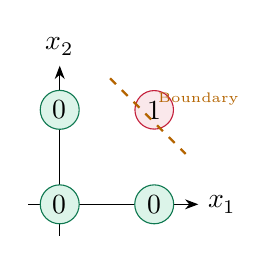
\begin{tikzpicture}[scale=0.8]
    \draw[-Stealth] (-0.5,0) -- (2.2,0) node[right] {$x_1$};
    \draw[-Stealth] (0,-0.5) -- (0,2.2) node[above] {$x_2$};
    \node[circle, draw=mygreen, fill=hdrgreen, inner sep=2pt] at (0,0) {$0$};
    \node[circle, draw=mygreen, fill=hdrgreen, inner sep=2pt] at (1.5,0) {$0$};
    \node[circle, draw=mygreen, fill=hdrgreen, inner sep=2pt] at (0,1.5) {$0$};
    \node[circle, draw=myred, fill=hdrred, inner sep=2pt] at (1.5,1.5) {$1$};
    \draw[dashed, thick, color=myamber] (0.8, 2.0) -- (2.0, 0.8) node[midway, above right] {\tiny Boundary};
  \end{tikzpicture}
  \par\vspace{2pt}\small\textbf{AND Gate (Linearly Separable)}
\end{minipage}
\hfill
\begin{minipage}{0.48\textwidth}
  \centering
  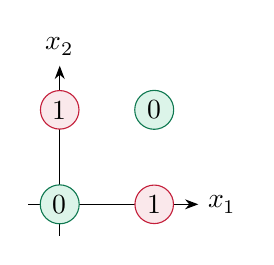
\begin{tikzpicture}[scale=0.8]
    \draw[-Stealth] (-0.5,0) -- (2.2,0) node[right] {$x_1$};
    \draw[-Stealth] (0,-0.5) -- (0,2.2) node[above] {$x_2$};
    \node[circle, draw=mygreen, fill=hdrgreen, inner sep=2pt] at (0,0) {$0$};
    \node[circle, draw=myred, fill=hdrred, inner sep=2pt] at (1.5,0) {$1$};
    \node[circle, draw=myred, fill=hdrred, inner sep=2pt] at (0,1.5) {$1$};
    \node[circle, draw=mygreen, fill=hdrgreen, inner sep=2pt] at (1.5,1.5) {$0$};
  \end{tikzpicture}
  \par\vspace{2pt}\small\textbf{XOR Gate (Non-Linearly Separable)}
\end{minipage}
\end{tcolorbox}

% ===============================================================================
\section{Hebb Net Learning Rule}
% ===============================================================================

Proposed by Donald Hebb in 1949, this is the oldest learning algorithm. It is based on the biological premise: *"Neurons that fire together, wire together."*

\begin{tcolorbox}[defbox, title={Hebbian Learning Rule}]
If two connected neurons are active simultaneously, the weight of the connection between them should be increased:
\begin{equation}
  w_i(\text{new}) = w_i(\text{old}) + x_i y
\end{equation}
where $x_i$ is the input and $y$ is the output.
\end{tcolorbox}

\subsection{Hebb Net Training Algorithm}
\begin{enumerate}[leftmargin=*, itemsep=2.5pt]
  \item Initialize all weights $w_i = 0$ and bias $b = 0$.
  \item For each training input vector $s = (s_1, s_2, \ldots, s_n)$ and target output $t$:
    \begin{itemize}[leftmargin=1.5em, itemsep=1.5pt]
      \item Set activation of input units $x_i = s_i$.
      \item Set activation of output unit $y = t$.
      \item Update weights: $w_i(\text{new}) = w_i(\text{old}) + x_i y$.
      \item Update bias: $b(\text{new}) = b(\text{old}) + y$.
    \end{itemize}
\end{enumerate}
\textit{Note: Hebb net learning works best when inputs and targets are represented in bipolar form ($\{-1, 1\}$) rather than binary form ($\{0, 1\}$).}

% ===============================================================================
\section{Perceptron Learning Algorithm}
% ===============================================================================

Developed by Frank Rosenblatt in 1958, the Perceptron is a supervised learning model used for binary classification.

\begin{tcolorbox}[formulabox, title={Perceptron Activation \& Weight Update}]
The output is computed using a binary/bipolar step activation:
\begin{equation}
  y = \begin{cases} 1 & \text{if } \sum w_i x_i + b \ge \theta \\ -1/0 & \text{if } \sum w_i x_i + b < \theta \end{cases}
\end{equation}
If the computed output $y$ does not match the target $t$, the weights and bias are updated using the Perceptron Learning Rule:
\begin{equation}
  w_i(\text{new}) = w_i(\text{old}) + \alpha (t - y) x_i
\end{equation}
\begin{equation}
  b(\text{new}) = b(\text{old}) + \alpha (t - y)
\end{equation}
where $\alpha \in (0, 1]$ is the learning rate.
\end{tcolorbox}

% ===============================================================================
\section{Adaline and Madaline Networks}
% ===============================================================================

\subsection{Adaline (Adaptive Linear Neuron)}
Developed by Widrow and Hoff (1960), Adaline is a single-element network that utilizes the Delta Rule (LMS - Least Mean Squares) for training.

\begin{tcolorbox}[defbox, title={Adaline vs. Perceptron}]
Unlike the Perceptron where weights are updated based on the thresholded binary output, Adaline updates weights using the continuous analog output \textbf{before} the activation function is applied.
\end{tcolorbox}

\par\noindent
The weight update in Adaline minimizes the mean squared error (gradient descent):
\begin{equation}
  w_i(\text{new}) = w_i(\text{old}) + \alpha (t - net) x_i
\end{equation}
where $net = \sum w_i x_i + b$ is the analog pre-activation sum.

\subsection{Madaline (Many Adalines)}
Madaline consists of a multilayer organization of Adaline units. The input layer connects to a hidden layer of Adaline units, which in turn connect to Madaline output units using fixed logic functions (AND, OR, or Majority vote). Madaline is trained using MRI (Madaline Rule I) or MRII algorithms.

% ===============================================================================
\section{Pattern Association Networks}
% ===============================================================================

Pattern association involves storing set of pattern pairs $(s^p, t^p)$ such that when an input pattern $s^p$ is presented, the network recalls the associated target pattern $t^p$.

\subsection{Classification of Associative Memories}
\begin{enumerate}[leftmargin=*, itemsep=3.5pt]
  \item \textbf{Auto-Associative Net:}
    A network where the input vector and target vector are identical ($s^p = t^p$). Its primary goal is pattern retrieval, denoising, or pattern completion. If a distorted or incomplete version of pattern $s^p$ is presented, the network outputs the original stored pattern $s^p$.
  \item \textbf{Hetero-Associative Net:}
    A network where the input vector and target vector are different ($s^p \neq t^p$, and they may reside in spaces of different dimensions). It maps an input vector in space $X$ to an associated target vector in space $Y$.
  \item \textbf{Iterative Auto-Associative Net:}
    A recurrent auto-associative network where output states are fed back as inputs dynamically. The network iteratively updates its activation values until it settles (converges) into a stable state representing one of the stored patterns (e.g., Hopfield networks).
\end{enumerate}

\subsection{Training Rules for Pattern Association}
Training an associative memory network involves constructing a weight matrix $W$ to map inputs to targets:
\begin{enumerate}[leftmargin=*, itemsep=3.5pt]
  \item \textbf{Hebbian Learning Rule (Outer Product Rule):}
    For $P$ bipolar pattern pairs $(s^p, t^p)$ where $s^p \in \{-1, 1\}^n$ and $t^p \in \{-1, 1\}^m$, the weight matrix is formed by summing the outer products of input-target pairs:
    \begin{equation}
      W = \sum_{p=1}^P (s^p)^T t^p \quad \implies \quad w_{ij} = \sum_{p=1}^P s_i^p t_j^p
    \end{equation}
  \item \textbf{Delta Rule (LMS / Widrow-Hoff Rule):}
    Used when patterns are not orthogonally separable. It is an iterative gradient descent rule that updates weights based on output error to minimize mean squared error:
    \begin{equation}
      \Delta w_{ij} = \alpha (t_j^p - y_j^p) s_i^p
    \end{equation}
    where $\alpha$ is the learning rate, $t_j^p$ is the target, and $y_j^p$ is the actual output.
\end{enumerate}

% ===============================================================================
\section{Bidirectional Associative Memory (BAM)}
% ===============================================================================

Introduced by Bart Kosko in 1988, BAM is a hetero-associative recurrent network that maps input vectors from space $X$ to target vectors in space $Y$.

\begin{tcolorbox}[formulabox, title={BAM Weight Matrix and Recall}]
Given $P$ bipolar pattern pairs $(S^p, T^p)$ where $S^p \in \{-1,1\}^n$ and $T^p \in \{-1,1\}^m$:
\par\noindent
The weight correlation matrix $W$ of size $n \times m$ is computed as:
\begin{equation}
  W = \sum_{p=1}^P (S^p)^T T^p
\end{equation}
\par\noindent
\textbf{Bidirectional Recall Process:}
\begin{itemize}[leftmargin=*, itemsep=3pt]
  \item \textbf{Forward Direction:} Feed input vector $X$ to recall output $Y$:
    \begin{equation}
      y_j = \text{sign}\left( \sum_{i=1}^n x_i w_{ij} \right) \quad \rightarrow \quad Y = \text{sign}(X W)
    \end{equation}
  \item \textbf{Backward Direction:} Feed output vector $Y$ back to recall input $X$:
    \begin{equation}
      x_i = \text{sign}\left( \sum_{j=1}^m y_j w_{ij} \right) \quad \rightarrow \quad X = \text{sign}(Y W^T)
    \end{equation}
\end{itemize}
\end{tcolorbox}

% ===============================================================================
\section{Worked Examples}
% ===============================================================================

\begin{tcolorbox}[examplebox, title={McCulloch-Pitts AND gate Implementation}]
\textbf{Problem:} Implement an AND gate using a McCulloch-Pitts neuron with binary inputs $x_1, x_2 \in \{0, 1\}$. Determine the weights and threshold $\theta$.
\par\vspace{4pt}\noindent\rule{\linewidth}{0.5pt}\par
\textbf{Solution:}
Let the weights be $w_1 = 1$, $w_2 = 1$ (excitatory weights).
The net input is $net = w_1 x_1 + w_2 x_2 = x_1 + x_2$.
The output equation is $y = 1$ if $net \ge \theta$, else $0$.
Let's construct the truth table and formulate inequalities for $\theta$:
\par\vspace{4pt}
\centering
{\renewcommand{\arraystretch}{1.65}%
\begin{tabular}{|c|c|c|c|l|}\hline
$x_1$ & $x_2$ & Target $t$ & $net = x_1 + x_2$ & Condition for threshold $\theta$ \\[4pt]
\hline
0 & 0 & 0 & 0 & $0 < \theta$ \\
\hline
1 & 0 & 0 & 1 & $1 < \theta$ \\
\hline
0 & 1 & 0 & 1 & $1 < \theta$ \\
\hline
1 & 1 & 1 & 2 & $2 \ge \theta$ \\
\hline
\end{tabular}
}
\par\vspace{4pt}\flushleft
From the table, the threshold $\theta$ must satisfy:
\begin{equation*}
  1 < \theta \le 2
\end{equation*}
Selecting $\theta = 2$ satisfies all conditions.
Thus, the M-P neuron with weights $w_1 = 1$, $w_2 = 1$ and threshold $\theta = 2$ implements the AND gate.
\end{tcolorbox}

\begin{tcolorbox}[examplebox, title={Hebb Net Weight Calculation}]
\textbf{Problem:} Train a Hebb net for the AND gate using bipolar inputs and targets.
\par\vspace{4pt}\noindent\rule{\linewidth}{0.5pt}\par
\textbf{Solution:}
The training patterns are:
$S^1 = (-1, -1), t^1 = -1$; \quad $S^2 = (1, -1), t^2 = -1$; \\
$S^3 = (-1, 1), t^3 = -1$; \quad $S^4 = (1, 1), t^4 = 1$.
\par\noindent
Initialize $w_1 = 0$, $w_2 = 0$, $b = 0$.
The weight update rules are: $\Delta w_1 = x_1 y$, $\Delta w_2 = x_2 y$, $\Delta b = y$.
\par\vspace{4pt}
\centering
{\renewcommand{\arraystretch}{1.65}%
\begin{tabular}{|c|c|c|c|c|c|c|c|c|}\hline
Step & $x_1$ & $x_2$ & $y$ & $\Delta w_1$ & $\Delta w_2$ & $w_1$ & $w_2$ & $b$ \\[4pt]
\hline
Init & -- & -- & -- & -- & -- & 0 & 0 & 0 \\
\hline
1 & -1 & -1 & -1 & 1 & 1 & 1 & 1 & -1 \\
\hline
2 & 1 & -1 & -1 & -1 & 1 & 0 & 2 & -2 \\
\hline
3 & -1 & 1 & -1 & 1 & -1 & 1 & 1 & -3 \\
\hline
4 & 1 & 1 & 1 & 1 & 1 & 2 & 2 & -2 \\
\hline
\end{tabular}
}
\par\vspace{4pt}\flushleft
The final weights are $w_1 = 2$, $w_2 = 2$ and bias $b = -2$.
The decision boundary is: $2 x_1 + 2 x_2 - 2 = 0 \implies x_1 + x_2 = 1$.
\end{tcolorbox}

\begin{tcolorbox}[examplebox, title={BAM Correlation Matrix Computation}]
\textbf{Problem:} Store the bipolar hetero-associative pattern pair $S = (1, -1, 1)$ and $T = (1, -1)$ in a BAM. Calculate the weight matrix $W$ and verify recall.
\par\vspace{4pt}\noindent\rule{\linewidth}{0.5pt}\par
\textbf{Solution:}
Given $S = \begin{bmatrix} 1 & -1 & 1 \end{bmatrix}$ and $T = \begin{bmatrix} 1 & -1 \end{bmatrix}$.
\par\noindent
The weight matrix is $W = S^T T$:
\begin{equation*}
  W = \begin{bmatrix} 1 \\ -1 \\ 1 \end{bmatrix} \begin{bmatrix} 1 & -1 \end{bmatrix} = \begin{bmatrix} 1 & -1 \\ -1 & 1 \\ 1 & -1 \end{bmatrix}
\end{equation*}
\par\noindent
\textbf{Verification of Forward Recall:}
Given input $S = \begin{bmatrix} 1 & -1 & 1 \end{bmatrix}$:
\begin{equation*}
  S W = \begin{bmatrix} 1 & -1 & 1 \end{bmatrix} \begin{bmatrix} 1 & -1 \\ -1 & 1 \\ 1 & -1 \end{bmatrix} = \begin{bmatrix} 1(1) + (-1)(-1) + 1(1) & 1(-1) + (-1)(1) + 1(-1) \end{bmatrix}
\end{equation*}
\begin{equation*}
  S W = \begin{bmatrix} 3 & -3 \end{bmatrix}
\end{equation*}
Applying the sign function:
\begin{equation*}
  Y = \text{sign}(S W) = \begin{bmatrix} \text{sign}(3) & \text{sign}(-3) \end{bmatrix} = \begin{bmatrix} 1 & -1 \end{bmatrix} = T \quad \textbf{(Verified)}
\end{equation*}
\end{tcolorbox}

\newpage

% ===============================================================================
% MANDATORY QUICK REVISION PAGE
% ===============================================================================
\begin{center}
  {\large\bfseries\color{myred} Quick Revision --- Module I}\\[3pt]
  {\small\color{mydark} Neural Networks and Pattern Association $|$ PE-EC702C}
\end{center}
\noindent{\color{myred}\rule{\linewidth}{1.2pt}}
\vspace{4pt}

\begin{tcolorbox}[formulabox, title={\textbf{Key Formulas at a Glance}}]
\renewcommand{\arraystretch}{1.3}
\begin{tabularx}{\linewidth}{B{5.0cm} X}M-P Neuron Output & $y = f\left(\sum w_i x_i\right) = \begin{cases} 1 & \text{if } \sum w_i x_i \ge \theta \\ 0 & \text{else} \end{cases}$ \\
Hebbian Learning & $w_i(\text{new}) = w_i(\text{old}) + x_i y, \quad b(\text{new}) = b(\text{old}) + y$ \\
Perceptron Learning Rule & $w_i(\text{new}) = w_i(\text{old}) + \alpha (t - y) x_i, \quad b(\text{new}) = b(\text{old}) + \alpha(t-y)$ \\
Adaline (LMS) Delta Rule & $w_i(\text{new}) = w_i(\text{old}) + \alpha (t - net) x_i \quad \text{where } net = \sum w_i x_i + b$ \\
BAM Weight Matrix & $W = \sum_{p=1}^P (S^p)^T T^p$ \\
BAM Bidirectional Recall & $Y = \text{sign}(X W), \quad X = \text{sign}(Y W^T)$
\end{tabularx}
\end{tcolorbox}

\begin{tcolorbox}[defbox, title={\textbf{One-Line Definitions}}]
\begin{itemize}[leftmargin=*, itemsep=2.5pt, topsep=0pt]
  \item \textbf{Activation Function:} A mathematical function that determines the neuron's output state based on its net input.
  \item \textbf{Linear Separability:} The property where data classes can be separated by a single hyperplane.
  \item \textbf{Hebbian Learning:} A learning paradigm where connection weights increase when pre- and post-synaptic units are active together.
  \item \textbf{Adaline:} A single-layer neural network trained using gradient descent to minimize mean squared output error.
  \item \textbf{BAM:} A hetero-associative recurrent neural network that stores bipolar vector pairs and performs bidirectional recall.
\end{itemize}
\end{tcolorbox}

\begin{tcolorbox}[exambox, title={\textbf{Frequently Asked / Viva Questions}}]
\begin{enumerate}[leftmargin=*, itemsep=3.5pt, label=\arabic*.]
  \item \Q{Compare biological and artificial neural networks in terms of speed and processing style.} Biological networks process information in a massively parallel, slow ($\sim$ms) style. ANNs process sequentially/quasi-parallelly but at extremely high electronic speeds ($\sim$ns).
  \item \Q{Explain the XOR problem in single-layer perceptrons.} Single-layer perceptrons can only classify linearly separable patterns. XOR inputs cannot be separated by a single decision boundary line, rendering them unclassifiable by single-layer perceptrons.
  \item \Q{What is the significance of the bias term in a neuron?} The bias acts as a shift factor for the activation function threshold, allowing the decision boundary to move away from the origin.
  \item \Q{What is the difference between Perceptron learning and Adaline learning?} Perceptron learning updates weights based on the thresholded binary output, whereas Adaline learning uses the continuous pre-activation sum (Delta rule).
  \item \Q{Define the stability-plasticity dilemma.} The dilemma of a network being stable enough to retain old learned patterns (stability) while remaining adaptive enough to learn new patterns (plasticity).
  \item \Q{Why is bipolar representation preferred over binary in Hebb nets?} In binary representation ($0,1$), inactive inputs ($0$) do not trigger weight updates, whereas bipolar representation ($-1,1$) allows learning from negative states.
  \item \Q{How does BAM retrieve stored patterns bidirectionally?} Inputs are multiplied by weight matrix $W$ to yield outputs, which are then multiplied by transpose matrix $W^T$ to retrieve inputs iteratively until stable convergence.
  \item \Q{What is the difference between supervised and unsupervised learning?} Supervised learning uses target outputs to adjust weights based on error feedback. Unsupervised learning groups data patterns based on similarity metrics without targets.
  \item \Q{What is the role of inhibitory inputs in the McCulloch-Pitts neuron?} Inhibitory inputs have absolute veto power: if an inhibitory input is active, the neuron output is forced to $0$ regardless of excitatory inputs.
  \item \Q{State the convergence theorem of perceptrons.} If the training data is linearly separable, the Perceptron learning algorithm is guaranteed to converge to a correct weight vector in a finite number of steps.
\end{enumerate}
\end{tcolorbox}

\begin{tcolorbox}[tikzbox, title={Comparison of Learning Rules}]
\centering
{\renewcommand{\arraystretch}{1.55}%
\begin{tabularx}{\linewidth}{|>{\bfseries}B{3.2cm}|Y|Y|}
\hline
Parameter & Hebbian Learning & Perceptron Learning \\
\hline
Learning Type & Unsupervised (self-association) & Supervised (target-based) \\
\hline
Weight Update Condition & Always updates based on activity & Updates only on classification error \\
\hline
Convergence Guarantee & No guarantee of convergence & Guaranteed convergence if linearly separable \\[4pt]
\hline
Feedback Loop & None & Error feedback loop present \\
\hline
\end{tabularx}}
\end{tcolorbox}

\end{document}
